\documentclass[tikz,border=3mm]{standalone}
\usetikzlibrary{positioning, shapes.geometric, arrows.meta, calc}

\begin{document}
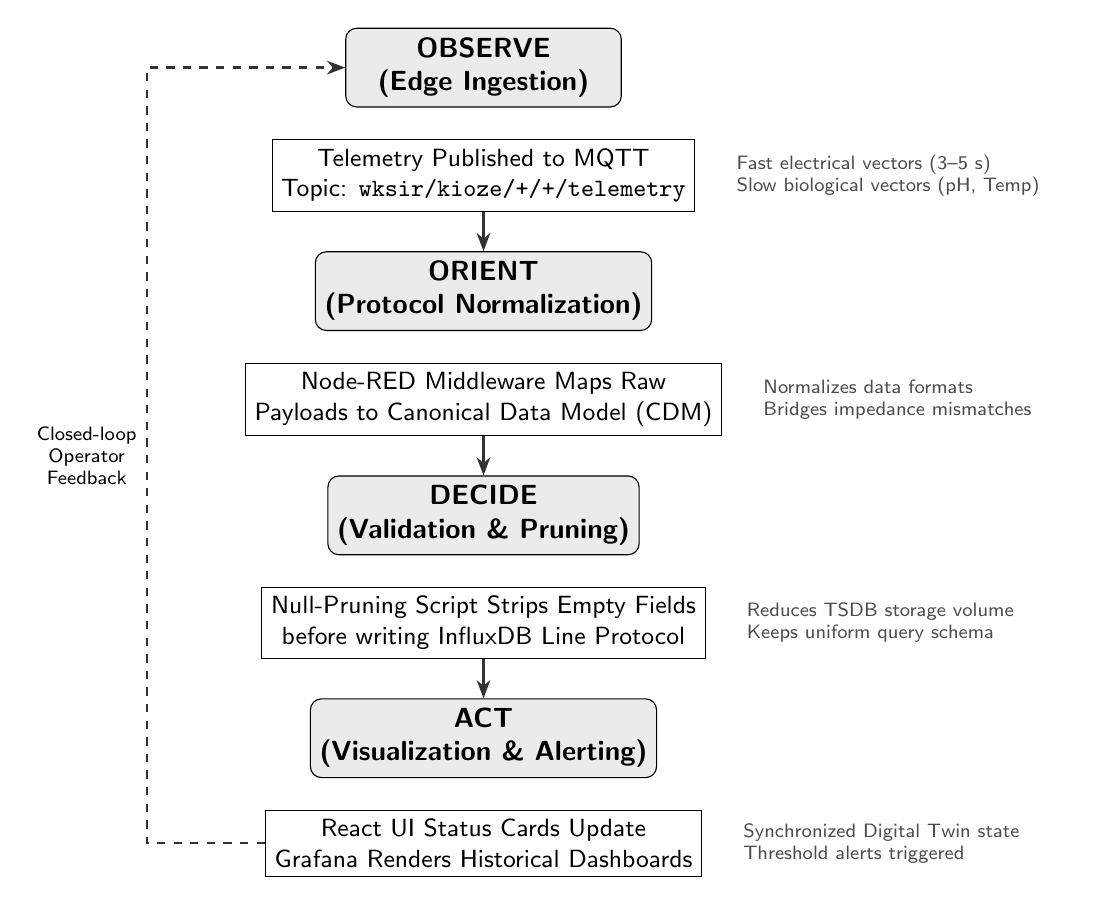
\begin{tikzpicture}[
    phase/.style={draw, fill=black!8, minimum width=3.5cm, minimum height=1cm, align=center, font=\bfseries\sffamily, shape=rectangle, rounded corners=4pt},
    stepbox/.style={draw, fill=white, minimum width=4.5cm, minimum height=0.8cm, align=center, font=\sffamily\small},
    arrow/.style={-Stealth, thick, draw=black!80},
    note/.style={text width=4cm, font=\sffamily\scriptsize, text=black!70}
]

    % Observe
    \node[phase] (P1) {OBSERVE\\(Edge Ingestion)};
    \node[stepbox, below=0.4cm of P1] (S1) {Telemetry Published to MQTT\\Topic: \texttt{wksir/kioze/+/+/telemetry}};
    \node[note, right=0.4cm of S1] (N1) {Fast electrical vectors (3--5 s)\\Slow biological vectors (pH, Temp)};

    % Orient
    \node[phase, below=0.5cm of S1] (P2) {ORIENT\\(Protocol Normalization)};
    \node[stepbox, below=0.4cm of P2] (S2) {Node-RED Middleware Maps Raw\\Payloads to Canonical Data Model (CDM)};
    \node[note, right=0.4cm of S2] (N2) {Normalizes data formats\\Bridges impedance mismatches};

    % Decide
    \node[phase, below=0.5cm of S2] (P3) {DECIDE\\(Validation \& Pruning)};
    \node[stepbox, below=0.4cm of P3] (S3) {Null-Pruning Script Strips Empty Fields\\before writing InfluxDB Line Protocol};
    \node[note, right=0.4cm of S3] (N3) {Reduces TSDB storage volume\\Keeps uniform query schema};

    % Act
    \node[phase, below=0.5cm of S3] (P4) {ACT\\(Visualization \& Alerting)};
    \node[stepbox, below=0.4cm of P4] (S4) {React UI Status Cards Update\\Grafana Renders Historical Dashboards};
    \node[note, right=0.4cm of S4] (N4) {Synchronized Digital Twin state\\Threshold alerts triggered};

    % Connectors
    \draw[arrow] (S1) -- (P2);
    \draw[arrow] (S2) -- (P3);
    \draw[arrow] (S3) -- (P4);
    
    % Loop feedback arrow
    \draw[arrow, dashed] (S4.west) -- ++(-1.5,0) |- (P1.west) node[pos=0.25, left, font=\sffamily\scriptsize, align=center] {Closed-loop\\Operator\\Feedback};

\end{tikzpicture}
\end{document}
